\documentclass{article}
\usepackage{txfonts}
\usepackage{tikz}
\usetikzlibrary{arrows,shapes,matrix}

\pagestyle{empty}
%
\tikzstyle{cblock}=[draw, fill=blue!20, minimum height=2em, text centered,
										inner sep= 0pt, text width= 4em, minimum width= 4em]
%\tikzstyle{init} = [pin edge={-to,thin,black}]

\tikzstyle{enc}=[draw, fill=blue!50, text centered, text width= 5em]
\tikzstyle{add}=[circle, draw, %fill=blue!20,
 inner sep=1pt]
\tikzstyle{mult}=[circle, draw,  inner sep=1pt]
\tikzstyle{ff} = [draw, inner sep = 1pt, minimum height=2em, minimum width=2em]
\begin{document}
\begin{figure}[b]
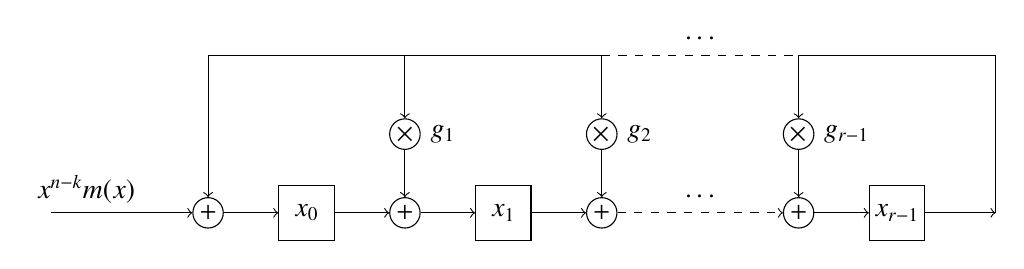
\begin{tikzpicture}[auto]

	
	    % Adders (XOR)
		\foreach \xpos/\lab in {0/a1, 2.5/a2, 5/a3, 7.5/a4}
		\node [add] (\lab) at (\xpos,0) {+};
		% Flip-flop or register 
		\foreach \xpos/\lab/\la in {1.25/0/r1, 3.75/1/r2, 8.75/{r-1}/r3}
		\node[ff] (\la) at (\xpos,0) {$x_{\lab}$};
		% Multipliers (AND)
		\node[mult, label={right:$g_1$}] (g1) at (2.5, 1) {$\times$};
		\node[mult, label={right:$g_2$}] (g2) at (5, 1) {$\times$};
		\node[mult, label={right:$g_{r-1}$}] (g3) at (7.5, 1) {$\times$};
		\foreach \xpos/\lab in {2.5/c1, 5/c2, 7.5/c3}
		\node[coordinate] (\lab) at (\xpos,2) {};
		
		\node[coordinate] (io) at (-2,0) {};
		\node[coordinate] (c0) at (0,2) {};
		\node[coordinate] (ct) at (10,0) {};
	
		\foreach \from/\to in {a1/r1, r1/a2, a2/r2, r2/a3, a4/r3, r3/ct}
		\draw[->] (\from) -- (\to) ;
		

		
	
	
		\draw[->] (a3) -- node[above] {$\cdots$} (a4) [dashed];
		%\draw (c0) -| (ct);
		\draw[->] (c0) -- (a1);
		\draw (c2) --  node[above] {$\cdots$} (c3) [dashed];
		\draw (c2) -- (c0) ;
		\draw (c3) -| (ct) ;
		\draw[->] (g1) -- (a2) ;
		\draw[->] (g2) -- (a3);
		\draw[->] (g3) -- (a4);
		\draw[->] (c1) -- (g1);
		\draw[->] (c2) -- (g2);
		\draw[->] (c3) -- (g3);
		\draw[->] (io) -- node[above,near start] {$x^{n-k}m(x)$}(a1);
\end{tikzpicture}
\end{figure}
\end{document}

